\section{安装Zookeeper}
\subsection{简介}
Zookeeper(动物管理员)相当于集群的管家,完成了集群中领导选举的工作,确保了集群中只有一个活跃的Master,避免了
“脑裂”现象。在Hadoop HA和HBase、Kafka等中均需要用到,一般来说都会在启动HDFS之前启动它。配置起来也不是很复杂。
\subsection{配置文件}
配置Zookeeper主要修改的文件就是\lstinline{conf\zoo.cfg}这个文件。
\begin{lstlisting}[style=mysh, title=zoo.cfg]
tickTime=2000
initLimit=5
syncLimit=2
# 上面3项保持默认即可
# zookeeper临时数据的保持目录,重要
dataDir=/home/zhangyu/zookeeperdata
# 连接端口,保持默认即可
clientPort=2181
#maxClientCnxns=60
# 这里需要配置3台服务器的地址
server.1=master:2888:8888
server.2=slave1:2888:8888
server.3=slave2:2888:8888
\end{lstlisting}
修改这个之后呢,还需要创建其中配置的\lstinline{dataDir=/home/zhangyu/zookeeperdata}
文件夹,并在其中创建一个文件\lstinline{myid},写入其id,要与\lstinline{server.x}
中对应。如Master是server1,则在myid文件中写1;Slave1是server2,则在myid文件中写2。

完成配置之后分别在各台机器上使用\lstinline{bin/zkServer.sh}启动服务即可。
\begin{lstlisting}[style=mysh]
$ zkServer.sh start
\end{lstlisting}
可以使用
\begin{lstlisting}[style=mysh]
$ zkServer.sh status
\end{lstlisting}
查看本机器状态,Leader或Follower。
同时使用Jps查看进程可以发现多了\lstinline{QuorumPeerMain}进程。

\subsection{zkCli命令行应用实践}

Zookeeper作为集群的管理者,在很多情况都会被用到,不光是Hadoop的HA机制,
包括后面可以看到Storm的HA机制、Kafka等的运行都要求前提是启动ZK集群。
在作为后台服务的协调集群的同时,Zookeeper还提供了zkCli.sh来方便查看集群中
的各个应用的健康信息。

\begin{center}
    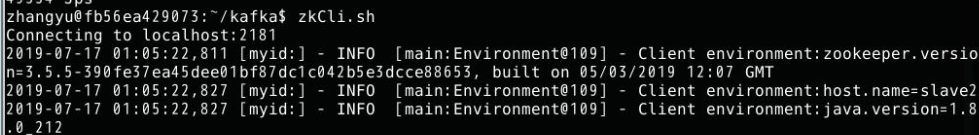
\includegraphics[width=\linewidth]{zookeeper/zkcli1.png}

    启动ZKCli进入命令行模式。

    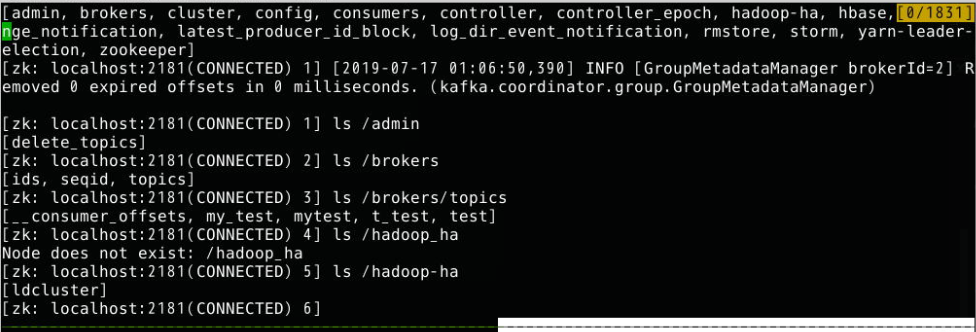
\includegraphics[width=\linewidth]{zookeeper/zkcli2.png}

    用类似Linux命令\lstinline{ls}查看运行的各个应用的信息。
\end{center}
